% Copyright (C) 2012 Raniere Silva
% 
% This file is part of 'CNPq 126874/2012-3'.
% 
% 'CNPq 126874/2012-3' is licensed under the Creative Commons
% Attribution 3.0 Unported License. To view a copy of this license,
% visit http://creativecommons.org/licenses/by/3.0/.
% 
% 'CNPq 126874/2012-3' is distributed in the hope that it will be
% useful, but WITHOUT ANY WARRANTY; without even the implied warranty of
% MERCHANTABILITY or FITNESS FOR A PARTICULAR PURPOSE.

\section{Método Preditor-Corretor}
Consideremos o problema de programação linear na forma padrão:
\begin{align*}
    \text{minimizar } & c^t x \\
    \text{sujeito a } & A x = b, \\
    & x \geq 0,
\end{align*}
onde $A \in \mathbb{R}^{m \times n}$ é uma matriz de posto completo $m$ e $c$,
$b$ e $x$ são vetores colunas de dimensão apropriada. Associado a este problema
temos o problema dual:
\begin{align*}
    \text{maximizar } & b^t y \\
    \text{sujeito a } & A^t y + z = c, \\
    & z \geq 0,
\end{align*}
onde $y$ é um vetor coluna de dimensão $m$ de variáveis livres e $z$ é o vetor
coluna de dimensão $n$ de variáveis de folga duais. O \textit{gap} dual é dado
por $\gamma = c^t x - b^t y$ que se reduz a $\gamma = x^t z$ para pontos primais
e duais factíveis.

A direção afim nos métodos de pontos interiores primais-duais é dada por:
\begin{align}
    \begin{bmatrix}
         0 & I & A^t \\
         Z & X & 0 \\
         A & 0 & 0
     \end{bmatrix} \begin{bmatrix}
         \tilde{x} \\
         \tilde{z} \\
         \tilde{y}
     \end{bmatrix} &= \begin{bmatrix}
         r_d \\
         r_a \\
         r_p
     \end{bmatrix},
     \label{eq:primal_dual_intp:lin_system}
\end{align}
onde $X = \diag(x)$, $Z = \diag(z)$ e os respiduos são dados por $r_p = b - A
x$, $r_d = c - A^t y - z$, $r_a = - X Z e$ e $e$ representa o vetor de uns.

Eliminando as variáveis $\tilde{z}$ de \eqref{eq:primal_dual_intp:lin_system}
obtemos o sistema aumentado:
\begin{align}
    \begin{bmatrix}
        -D & A^t \\
        A & 0
    \end{bmatrix} \begin{bmatrix}
        \tilde{x} \\
        \tilde{y}
    \end{bmatrix} &= \begin{bmatrix}
        r_1 \\
        r_2
    \end{bmatrix},
    \label{eq:primal_dual_intp:aug_lin_system}
\end{align}
onde $D = X^{-1} Z$.

A forma mais utilizada para resolver \eqref{eq:primal_dual_intp:aug_lin_system}
consiste em reduzir o sistema através de eliminção das variáveis $\tilde{x}$ a
um sistema simétrico definido positivo com a matriz de equações normais $A
D^{-1} A^t$ e aplicar então a fatoração de Cholesky.

\section{Matrizes}
\subsection{Matrizes Esparsas}
Uma matriz é dita esparsa quando a maioria de seus elementos são iguais a zero, ou seja, ela possui relativamente poucos elementos não nulos. Sistemas lineares que surgem na solução de problemas reais possuem, em sua maioria, matrizes esparsas e de ordem elevada. Nestes casos, é proibitivo armazenar toda a matriz por questão de memória do computador e o que se faz na prática é guardar somente os elementos não nulos.

Uma matriz é dita simétrica quando $A_{ij} = A_{ji}$.

\begin{figure}[!htb]
    \centering
    \begin{tikzpicture}
        \matrix (A) [matrix of math nodes,%
        left delimiter  = (,%
        right delimiter = )] at (0,0)
        {%
        X & X & X & X & X & 0 & 0 \\
        X & X & 0 & 0 & 0 & X & X \\
        X & 0 & X & 0 & 0 & X & X \\
        X & 0 & 0 & X & 0 & 0 & 0 \\
        X & 0 & 0 & 0 & X & 0 & 0 \\
        0 & X & X & 0 & 0 & X & 0 \\
        0 & X & X & 0 & 0 & 0 & X \\
        };
        \node[above, shift={(0,.5)}] at (A-1-1) {$1$};
        \node[above, shift={(0,.5)}] at (A-1-2) {$2$};
        \node[above, shift={(0,.5)}] at (A-1-3) {$3$};
        \node[above, shift={(0,.5)}] at (A-1-4) {$4$};
        \node[above, shift={(0,.5)}] at (A-1-5) {$5$};
        \node[above, shift={(0,.5)}] at (A-1-6) {$6$};
        \node[above, shift={(0,.5)}] at (A-1-7) {$7$};
        \node[right, shift={(-1.5,0)}] at (A-1-1) {$1$};
        \node[right, shift={(-1.5,0)}] at (A-2-1) {$2$};
        \node[right, shift={(-1.5,0)}] at (A-3-1) {$3$};
        \node[right, shift={(-1.5,0)}] at (A-4-1) {$4$};
        \node[right, shift={(-1.5,0)}] at (A-5-1) {$5$};
        \node[right, shift={(-1.5,0)}] at (A-6-1) {$6$};
        \node[right, shift={(-1.5,0)}] at (A-7-1) {$7$};

        \matrix (B) [matrix of math nodes,%
        left delimiter  = (,%
        right delimiter = )] at (8,0)
        {%
        X & 0 & X & X & 0 & 0 & 0 \\
        0 & X & X & X & 0 & 0 & 0 \\
        X & X & X & 0 & X & 0 & 0 \\
        X & X & 0 & X & X & 0 & 0 \\
        0 & 0 & X & X & X & X & X \\
        0 & 0 & 0 & 0 & X & X & 0 \\
        0 & 0 & 0 & 0 & X & 0 & X \\
        };
        \node[above, shift={(0,.5)}] at (B-1-1) {$1$};
        \node[above, shift={(0,.5)}] at (B-1-2) {$2$};
        \node[above, shift={(0,.5)}] at (B-1-3) {$3$};
        \node[above, shift={(0,.5)}] at (B-1-4) {$4$};
        \node[above, shift={(0,.5)}] at (B-1-5) {$5$};
        \node[above, shift={(0,.5)}] at (B-1-6) {$6$};
        \node[above, shift={(0,.5)}] at (B-1-7) {$7$};
        \node[right, shift={(-1.5,0)}] at (B-1-1) {$1$};
        \node[right, shift={(-1.5,0)}] at (B-2-1) {$2$};
        \node[right, shift={(-1.5,0)}] at (B-3-1) {$3$};
        \node[right, shift={(-1.5,0)}] at (B-4-1) {$4$};
        \node[right, shift={(-1.5,0)}] at (B-5-1) {$5$};
        \node[right, shift={(-1.5,0)}] at (B-6-1) {$6$};
        \node[right, shift={(-1.5,0)}] at (B-7-1) {$7$};
    \end{tikzpicture}
    \caption{Exemplos de matriz simétrica.}
    \label{fig:exem_matriz_simetrica}
\end{figure}

A largura de banda, $\beta$, de uma matriz simétrica $A \in \mathbb{R}^{n \times n}$ é dada pela maior distância de um elemento não nulo à diagonal principal, ou seja:
\begin{align*}
    \beta(A) &= \max_{a_{ij} \neq 0} | i - j |.
\end{align*}

\begin{figure}[!htb]
    \centering
    \begin{tikzpicture}
        \matrix (A) [matrix of math nodes,%
        left delimiter  = (,%
        right delimiter = )] at (0,0)
        {%
        X & X & X & X & X & 0 & 0 \\
        X & X & 0 & 0 & 0 & X & X \\
        X & 0 & X & 0 & 0 & X & X \\
        X & 0 & 0 & X & 0 & 0 & 0 \\
        X & 0 & 0 & 0 & X & 0 & 0 \\
        0 & X & X & 0 & 0 & X & 0 \\
        0 & X & X & 0 & 0 & 0 & X \\
        };
        \node[above, shift={(0,.5)}] at (A-1-1) {$1$};
        \node[above, shift={(0,.5)}] at (A-1-2) {$2$};
        \node[above, shift={(0,.5)}] at (A-1-3) {$3$};
        \node[above, shift={(0,.5)}] at (A-1-4) {$4$};
        \node[above, shift={(0,.5)}] at (A-1-5) {$5$};
        \node[above, shift={(0,.5)}] at (A-1-6) {$6$};
        \node[above, shift={(0,.5)}] at (A-1-7) {$7$};
        \node[right, shift={(-1.5,0)}] at (A-1-1) {$1$};
        \node[right, shift={(-1.5,0)}] at (A-2-1) {$2$};
        \node[right, shift={(-1.5,0)}] at (A-3-1) {$3$};
        \node[right, shift={(-1.5,0)}] at (A-4-1) {$4$};
        \node[right, shift={(-1.5,0)}] at (A-5-1) {$5$};
        \node[right, shift={(-1.5,0)}] at (A-6-1) {$6$};
        \node[right, shift={(-1.5,0)}] at (A-7-1) {$7$};
        % Largura de banda
        \draw (A-1-6.north east) -- (A-2-7.north east);
        \draw (A-6-1.south west) -- (A-7-2.south west);

        \matrix (B) [matrix of math nodes,%
        left delimiter  = (,%
        right delimiter = )] at (8,0)
        {%
        X & 0 & X & X & 0 & 0 & 0 \\
        0 & X & X & X & 0 & 0 & 0 \\
        X & X & X & 0 & X & 0 & 0 \\
        X & X & 0 & X & X & 0 & 0 \\
        0 & 0 & X & X & X & X & X \\
        0 & 0 & 0 & 0 & X & X & 0 \\
        0 & 0 & 0 & 0 & X & 0 & X \\
        };
        \node[above, shift={(0,.5)}] at (B-1-1) {$1$};
        \node[above, shift={(0,.5)}] at (B-1-2) {$2$};
        \node[above, shift={(0,.5)}] at (B-1-3) {$3$};
        \node[above, shift={(0,.5)}] at (B-1-4) {$4$};
        \node[above, shift={(0,.5)}] at (B-1-5) {$5$};
        \node[above, shift={(0,.5)}] at (B-1-6) {$6$};
        \node[above, shift={(0,.5)}] at (B-1-7) {$7$};
        \node[right, shift={(-1.5,0)}] at (B-1-1) {$1$};
        \node[right, shift={(-1.5,0)}] at (B-2-1) {$2$};
        \node[right, shift={(-1.5,0)}] at (B-3-1) {$3$};
        \node[right, shift={(-1.5,0)}] at (B-4-1) {$4$};
        \node[right, shift={(-1.5,0)}] at (B-5-1) {$5$};
        \node[right, shift={(-1.5,0)}] at (B-6-1) {$6$};
        \node[right, shift={(-1.5,0)}] at (B-7-1) {$7$};
        % Largura de banda
        \draw (B-1-4.north east) -- (B-4-7.north east);
        \draw (B-4-1.south west) -- (B-7-4.south west);
    \end{tikzpicture}
    \caption{Exemplos da largura de banda para matriz simétrica.}
    \label{fig:exem_bandwidth}
\end{figure}
% TODO Escrever melhor
É possível ``generalizar'' a largura de banda para cada linha da matiz simética

O envelope, $\rho$, da matriz é dado por
\begin{align*}
    \rho(A) = \sum_{i = 1}^n \beta_i(A).
\end{align*}

\begin{figure}[!htb]
    \centering
    \begin{tikzpicture}
        \matrix (A) [matrix of math nodes,%
        left delimiter  = (,%
        right delimiter = )] at (0,0)
        {%
        X & X & X & X & X & 0 & 0 \\
        X & X & 0 & 0 & 0 & X & X \\
        X & 0 & X & 0 & 0 & X & X \\
        X & 0 & 0 & X & 0 & 0 & 0 \\
        X & 0 & 0 & 0 & X & 0 & 0 \\
        0 & X & X & 0 & 0 & X & 0 \\
        0 & X & X & 0 & 0 & 0 & X \\
        };
        \node[above, shift={(0,.5)}] at (A-1-1) {$1$};
        \node[above, shift={(0,.5)}] at (A-1-2) {$2$};
        \node[above, shift={(0,.5)}] at (A-1-3) {$3$};
        \node[above, shift={(0,.5)}] at (A-1-4) {$4$};
        \node[above, shift={(0,.5)}] at (A-1-5) {$5$};
        \node[above, shift={(0,.5)}] at (A-1-6) {$6$};
        \node[above, shift={(0,.5)}] at (A-1-7) {$7$};
        \node[right, shift={(-1.5,0)}] at (A-1-1) {$1$};
        \node[right, shift={(-1.5,0)}] at (A-2-1) {$2$};
        \node[right, shift={(-1.5,0)}] at (A-3-1) {$3$};
        \node[right, shift={(-1.5,0)}] at (A-4-1) {$4$};
        \node[right, shift={(-1.5,0)}] at (A-5-1) {$5$};
        \node[right, shift={(-1.5,0)}] at (A-6-1) {$6$};
        \node[right, shift={(-1.5,0)}] at (A-7-1) {$7$};
        % Perfil
        \draw[fill=gray, fill opacity=0.2] (A-1-1.north west) -- (A-6-1.north
        west) -- (A-6-2.north west) --
        (A-7-2.south west)
        \foreach \x in {7,6,5,4,3,2,1}{
        -- (A-\x-\x.south east) -- (A-\x-\x.north east) -- (A-\x-\x.north west)
        };

        \matrix (B) [matrix of math nodes,%
        left delimiter  = (,%
        right delimiter = )] at (8,0)
        {%
        X & 0 & X & X & 0 & 0 & 0 \\
        0 & X & X & X & 0 & 0 & 0 \\
        X & X & X & 0 & X & 0 & 0 \\
        X & X & 0 & X & X & 0 & 0 \\
        0 & 0 & X & X & X & X & X \\
        0 & 0 & 0 & 0 & X & X & 0 \\
        0 & 0 & 0 & 0 & X & 0 & X \\
        };
        \node[above, shift={(0,.5)}] at (B-1-1) {$1$};
        \node[above, shift={(0,.5)}] at (B-1-2) {$2$};
        \node[above, shift={(0,.5)}] at (B-1-3) {$3$};
        \node[above, shift={(0,.5)}] at (B-1-4) {$4$};
        \node[above, shift={(0,.5)}] at (B-1-5) {$5$};
        \node[above, shift={(0,.5)}] at (B-1-6) {$6$};
        \node[above, shift={(0,.5)}] at (B-1-7) {$7$};
        \node[right, shift={(-1.5,0)}] at (B-1-1) {$1$};
        \node[right, shift={(-1.5,0)}] at (B-2-1) {$2$};
        \node[right, shift={(-1.5,0)}] at (B-3-1) {$3$};
        \node[right, shift={(-1.5,0)}] at (B-4-1) {$4$};
        \node[right, shift={(-1.5,0)}] at (B-5-1) {$5$};
        \node[right, shift={(-1.5,0)}] at (B-6-1) {$6$};
        \node[right, shift={(-1.5,0)}] at (B-7-1) {$7$};
        % Perfil
        \draw[fill=gray, fill opacity=0.2] (B-1-1.north west) -- (B-5-1.north
        west) -- (B-5-3.north west) --
        (B-5-3.south west) -- (B-6-5.north west) -- (B-7-5.south west)
        \foreach \x in {7,6,5,4,3,2,1}{
        -- (B-\x-\x.south east) -- (B-\x-\x.north east) -- (B-\x-\x.north west)
        };
    \end{tikzpicture}
    \caption{Exemplos da largura de banda para matriz simétrica.}
    \label{fig:exem_profile}
\end{figure}

\subsection{Grafos e matrizes esparsas}
A teoria dos grafos foi identificada como uma poderosa ferramenta para a computação de matrizes esparsas quando Seymour Parter [Par61] usou grafos não direcionados para modelar a eliminação Gaussiana há mais de quarenta anos atrás. Grafos podem ser usados para modelar matrizes simítricas, não simétricas, fatorações etc. Além de tornar mais fácil a compreensão e análise de algoritmos para matrizes esparsas, eles também aumentam o escopo de manipulações destas matrizes usando algoritmos e técnicas já existentes.

Um grafo é, fundamentalmente, um modo de representar uma relação binária entre objetos. Para o propósito deste trabalho, considere um grafo $G = (V, E)$ como um conjunto de vértices $V = \{v_1, v_2, \ldots \}$ (ou nós) e um conjunto de arestas $E = \{e_1, e_2, \ldots \}$. Estas arestas são representadas por pares não ordenados, por exemplo, $e_1 = (v_1 , v_2)$.

Um conhecimento básico de teoria dos grafos é importante para o entendimento do trabalho. Conceitos mais específicos serão introduzidos quando necessários. Um resumo dos principais conceitos é dado por:
\begin{description}
    \item[Grau do vértice] número de arestas incidentes no vértice.
    \item[Vértices adjacentes]  dois vértices $v_1$ e $v_2$ são adjacentes quando possue uma aresta entre eles, ou seja, $e_1 = (v_1, v_2)$.
    \item[Caminho] sequência de arestas disjuntas $\left( (x_1, x_2), (x_2, x_3), \ldots (x_{k - 1}, x_k) \right)$.
    \item[Grafo conectado (conexo)] possui caminho entre qualquer par de vértices.
    \item[Subgrafo completo (clique)] cada vértice do subgrafo possue aresta incidente em todos os outros vértices do subgrafo.
    \item[Árvore] grafo conectado sem ciclos.
\end{description}

Assim como um grafo, uma matriz tambm descreve uma relação binária entre variáveis através de seus elementos não nulos. Uma matriz simétrica $A_{n \times n}$ pode ser modelada como um grafo $G(V, E)$, onde os $n$ vértices em $V$ representam as dimensões da matriz e existe uma aresta conectando os vértices $i$ e $j$ se $a_{ij} = 0$.

\begin{figure}[!htb]
    \centering
    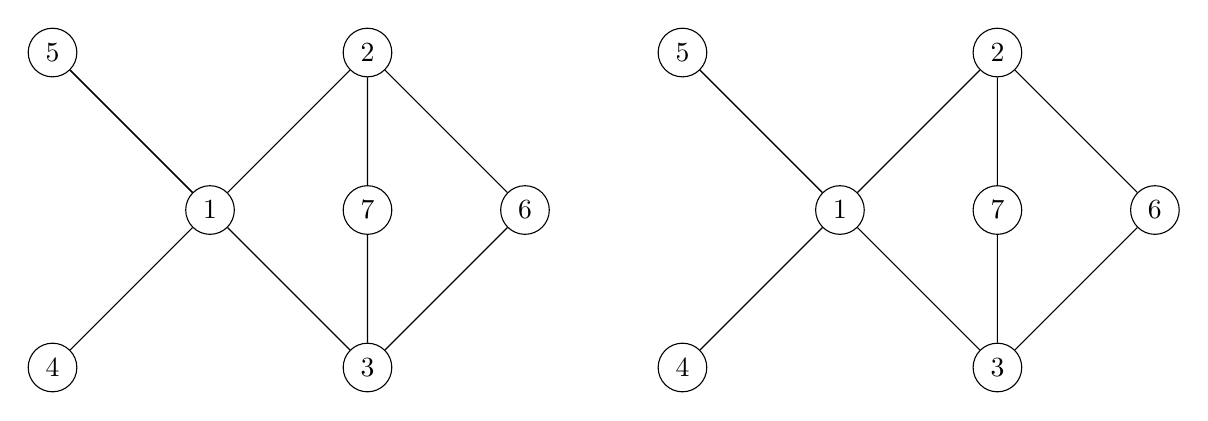
\begin{tikzpicture}
        \node[draw, circle] (A1) at (0,0) {1};
        \node[draw, circle] (A5) at (-2,2) {5};
        \node[draw, circle] (A4) at (-2,-2) {4};
        \node[draw, circle] (A2) at (2,2) {2};
        \node[draw, circle] (A3) at (2,-2) {3};
        \node[draw, circle] (A6) at (2,0) {7};
        \node[draw, circle] (A7) at (4,0) {6};
        \draw (A1) -- (A5) (A1) -- (A4) (A1) -- (A2);
        \draw (A1) -- (A5) (A2) -- (A7) (A3) -- (A7);
        \draw (A2) -- (A6) (A3) -- (A6) (A1) -- (A3);

        \node[draw, circle] (B1) at (8,0) {1};
        \node[draw, circle] (B5) at (6,2) {5};
        \node[draw, circle] (B4) at (6,-2) {4};
        \node[draw, circle] (B2) at (10,2) {2};
        \node[draw, circle] (B3) at (10,-2) {3};
        \node[draw, circle] (B6) at (10,0) {7};
        \node[draw, circle] (B7) at (12,0) {6};
        \draw (B1) -- (B5) (B1) -- (B4) (B1) -- (B2);
        \draw (B1) -- (B5) (B2) -- (B7) (B3) -- (B7);
        \draw (B2) -- (B6) (B3) -- (B6) (B1) -- (B3);
    \end{tikzpicture}
    \caption{Exemplos do grafo correspondente a matriz simétrica.}
    \label{fig:exem_graph}
\end{figure}
\subsection{Fatoração de matrizes esparsas}
Considerando
\begin{align*}
    A &= \begin{bmatrix}
        1 & 1 & 1 & 1 & 1 & 0 & 0 \\
        1 & 1 & 0 & 0 & 0 & 1 & 1 \\
        1 & 0 & 1 & 0 & 0 & 1 & 1 \\
        1 & 0 & 0 & 1 & 0 & 0 & 0 \\
        1 & 0 & 0 & 0 & 1 & 0 & 0 \\
        0 & 1 & 1 & 0 & 0 & 1 & 0 \\
        0 & 1 & 1 & 0 & 0 & 0 & 1
    \end{bmatrix},
\end{align*}
verifica-se que
\begin{align*}
    U &= \begin{bmatrix}
        1 &    1 &    1 &    1 &    1 &    0 &    0 \\
        0 &   -1 &    0 &   -1 &   -1 &    1 &    1 \\
        0 &    0 &   -1 &   -1 &   -1 &    1 &    1 \\
        0 &    0 &    0 &    2 &    1 &   -2 &   -2 \\
        0 &    0 &    0 &    0 &  3/2 &   -1 &   -1 \\
        0 &    0 &    0 &    0 &    0 & -2/3 &  1/3 \\
        0 &    0 &    0 &    0 &    0 &    0 & -1/2
    \end{bmatrix},
\end{align*}
onde $A = P L U$.

Permutando linhas e colunas de $A$ tal que
\begin{align*}
    A' &= \begin{bmatrix}
        1 & 0 & 1 & 1 & 0 & 0 & 0 \\
        0 & 1 & 1 & 1 & 0 & 0 & 0 \\
        1 & 1 & 1 & 0 & 1 & 0 & 0 \\
        1 & 1 & 0 & 1 & 1 & 0 & 0 \\
        0 & 0 & 1 & 1 & 1 & 1 & 1 \\
        0 & 0 & 0 & 0 & 1 & 1 & 0 \\
        0 & 0 & 0 & 0 & 1 & 0 & 1
    \end{bmatrix},
\end{align*}
verifica-se que
\begin{align*}
    U' &= \begin{bmatrix}
        1 &    0 &    1 &    1 &    0 &    0 &    0 \\
        0 &    1 &    1 &    1 &    0 &    0 &    0 \\
        0 &    0 &   -2 &   -1 &    1 &    0 &    0 \\
        0 &    0 &    0 & -3/2 &  1/2 &    0 &    0 \\
        0 &    0 &    0 &    0 &  5/3 &    1 &    1 \\
        0 &    0 &    0 &    0 &    0 & -3/5 &  2/5 \\
        0 &    0 &    0 &    0 &    0 &    0 & -1/3
    \end{bmatrix}.
\end{align*}
onde $A' = P' L' U'$.

Comparando $U$ e $U'$ verifica-se que o número de elementos nulos na parte
triangular superior da matriz $U'$ é maior na matriz $U$. E
comparando os elementos nulos na parte triangular superior de $A'$ e $U'$
verifica-se que apenas o elemento $A'_{34}$ deixou de ser nulo
enquanto que em relação a $A$ e $U$ apenas os elementos $A_{16}$,
$A_{17}$ e $A_{23}$ permaneceram nulos.
comparamos os elementos 

Pelo exemplo anterior, verifica-se a possibilidade de pré-processar a matrix
de forma a reduzir a complexidade da resolução do sistema linear. Alguns
exemplos de pré-processamentos indicados por Ghidetti
\cite{Ghidetti:2010:ComparativoReordenamento} são a minimização da
largura de banda e a redução do envelope ou \textit{profile}. ``Esses
pré-processamentos consistem em dispor os elementos não nulos da matriz o mais
próximo possível da diagonal principal.''

``No contexto da solução de sisteas lineares via métodos diretos, a
minimização da largura da bnada pode proporcionar uma redução no
preenchimento que ocorre na decomposição. (\ldots) Contudo, atualmente
sistemas lineares de grande pore são usualmente solucionados por métodos
iterativos não estacionários que por um lado não alteram a esparsidade da
matriz, mas necessitam de critérios de convergência. Em geral, um
processo para acelerar a convergência, denominado precondicionamento, se faz
necessário. Os precondicionadores baseados na decomposição LU são
amplamente utilizados por apresentar uma taxa acentuada na aceleração da
convergência. Porém, tais operações alteram a esparsidade da matriz e
portanto um processo de reordenamento da matriz é fundamental para a
eficiência de tais precondicionadores.''

\section{Cuthill-McKee reverso}
No Método Preditor-Corretor pode-se utilizar a Decomposição de Cholesky para resolver o sistema linear
% TODO Identificar o sistema linear do Método Preditor-Corretor

Para problemas de grande porte, esse sistema linear é esparso e ao utilizar a Decomposição de Cholesky pode ocorrer o preenchimento da matriz.
% TODO Incluir exemplo.

É possivel permutar linhas e colunas do sistema linear de modo a minimizar o preenchimento decorrente da Decomposição de Choleslky.
% TODO Incluir exemplo.

Cuthill e McKee \cite{Cuthill:1969:ReducingBandwidth} propuseram um algoritmo de reordenação, cujo objetivo principal é reduzir a largura de banda de uma matriz simétrica.

% TODO Mostrar equivalência com grafos
\begin{algorithm}
    \caption{Pseudo-algoritmo RCM}
    \label{alg:rcm}
    \begin{algorithmic}
        \REQUIRE Grafo $G(A)$ e um vértice $v$ de grau mínimo.
        \ENSURE $n$, novo ordenamento dos vértices de $G(A)$.
        \STATE $p = \text{ vetor de zeros}$
        \STATE $n = \text{ vetor de zeros}$
        \STATE $i = 1$
        \STATE $f = \text{ fila vazia}$
        \STATE Enfileira $v$ em $f$
        \STATE $p_v = 1$
        \WHILE{$f$ não for vazia}
            \STATE Desenfeira $f$ em $v$
            \STATE $n_v = i$
            \STATE $i = i + 1$
            \FOR{vertice $w$ adjacente a $v$}
                \IF{$p_w == 0$}
                    \STATE Enfileira $w$ em $f$
                    \STATE $p_w = 1$
                \ENDIF
            \ENDFOR
        \ENDWHILE
    \end{algorithmic}
\end{algorithm}
